\documentclass{beamer}
\usepackage{graphicx}
\usepackage{listings}
\lstset{
basicstyle=\small\ttfamily,
columns=flexible,
breaklines=true
}
\usepackage{url}
\usepackage[colorinlistoftodos]{todonotes}
%Information to be included in the title page:
\title{Haskell or How I Learned to Stop Worrying and Love in General: Haskell for Flow Cytometry}
\author{Noah Thomas Jones}
\institute{University of Florida}
\date{}
\begin{document}
\frame{\titlepage}
\begin{frame}
  \frametitle{What is Flow?}
  \begin{figure}
    \centering
    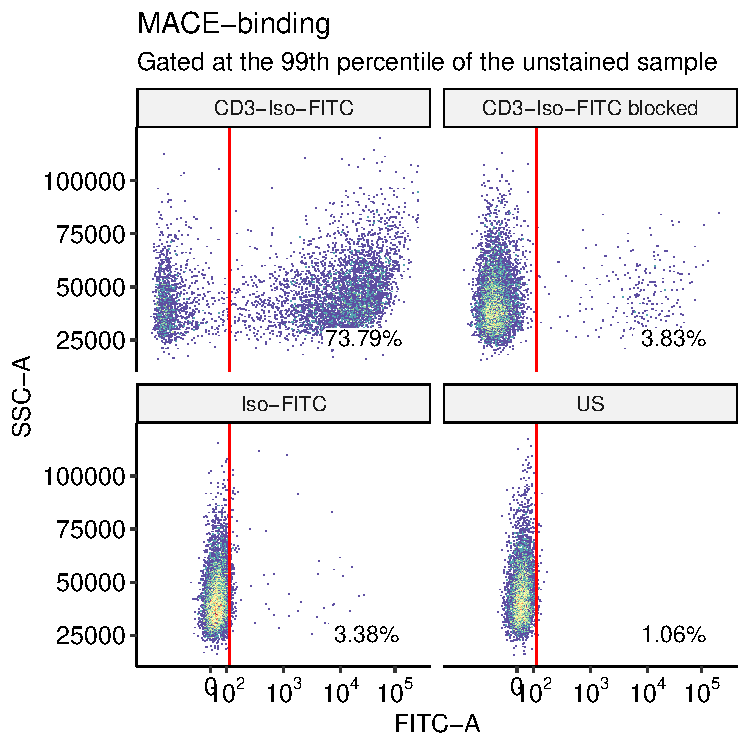
\includegraphics[width=0.45\textwidth]{./images/NJ030_MACE-binding.pdf}
    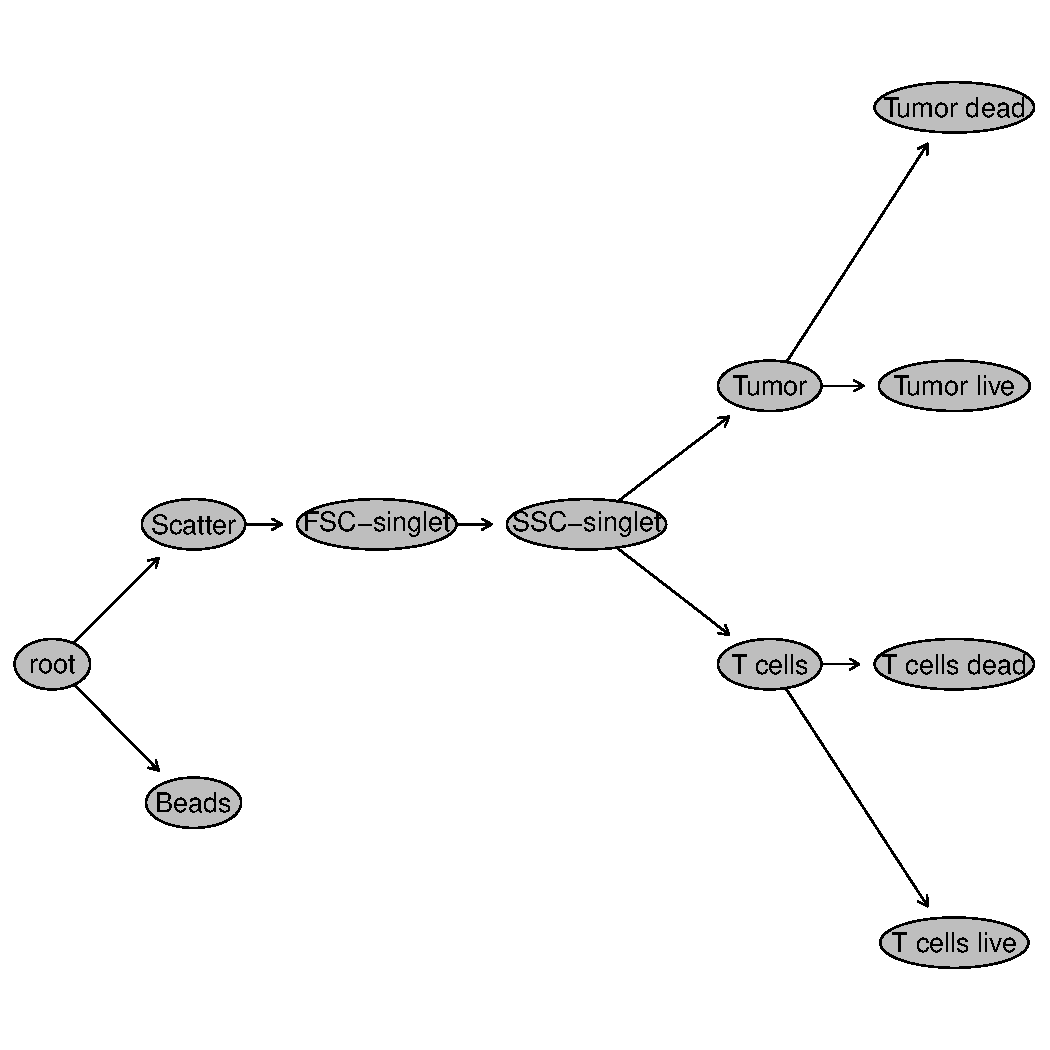
\includegraphics[width=0.45\textwidth]{./images/NJ017_gates.pdf}
    \caption{Examples: gates on fluorescent channels and
      example gating scheme.}
  \end{figure}
\end{frame}
\begin{frame}
  \frametitle{Problem Statement}
  We need flow cytometry gating scheme that does not
\end{frame}
\begin{frame}[fragile]
  \frametitle{Existing Solutions} We have a gating ML
  standard\cite{spidlen2015isac}, which does something for portability
  of gates, but of the tools used, one notable example is the R
  library \texttt{flowCore}, which after defining a \texttt{gatingset} object,
  which is an object tenuously linked to a \texttt{flowset} object, is
  modified through imperative side-effects.
\begin{lstlisting}
rg1 <- rectangleGate("FSC-A"=c(50000, Inf), filterId="NonDebris")
gs_pop_add(gs, rg1, parent = "root")
## [1] 2
gs_get_pop_paths(gs)
## [1] "root" "/NonDebris"
# gate the data
recompute(gs)
## done!
\end{lstlisting}
\end{frame}

\begin{frame}[fragile]
  \frametitle{Getting Started} The first objective was to write a file
  parser so that we can pull data out of our files. We can start based
  on our file specification\cite{spidlen2021data}.
\end{frame}
\begin{frame}[fragile]
  \frametitle{FCS3.0}
  Basic info:
  \begin{enumerate}
  \item Established in 1996 by the International Society for
    Analytical Cytology (ISAC) Data File Standards Committee
    \cite{standards1996}.
  \item Significant changes include:
    \begin{enumerate}
    \item a mechanism for handling data sets of 100 megabytes and larger, 
    \item support for UNICODE text for keyword values, and 
    \item support for cyclic redundancy check (CRC) validation for
      each data set.
    \end{enumerate}
  \end{enumerate}
  Here is an example header:
  \begin{lstlisting}
    FCS3.0         256    1545    1792  202456       0       0 
  \end{lstlisting}
\end{frame}

\begin{frame}[fragile]
  \frametitle{FCS3.0}
  Here a condensed paraphrase of the header specification:\todo[inline]{Condense to fit slide}
  \begin{enumerate}
  \item The HEADER segment begins at byte offset zero. 
  \item The first six bytes in the HEADER segment comprise the version identifier (FCS3.0).
  \item The next 4 bytes (6 - 9) are occupied by space characters (ASCII 32). 
  \item Following the identifier are at least three pairs of ASCII-encoded integers indicating the byte offsets for the start and end of the
    \begin{enumerate}
    \item primary TEXT segment, 
    \item the DATA segment, and the 
    \item ANALYSIS segment, respectively.
    \end{enumerate}
  \item The byte offsets are referenced to the beginning of the data set.
  \end{enumerate}
\end{frame}
\begin{frame}
  \frametitle{FCS3.0 Byte Offsets}
  \begin{enumerate}
  \item Under FCS3.0 these offsets remain limited to 8 bytes. 
  \item Each ASCII encoded integer offset is right justified in its 8 byte space. 
  \item Offset locations (bytes):
    \begin{enumerate}
    \item [10--17] start of the primary TEXT segment
    \item [18--25] end of the primary TEXT segment
    \item [26--33] start of the DATA segment
    \item [34--41] end of the DATA segment
    \item [42--49] start of the ANALYSIS segment
    \item [50--57] end of the ANALYSIS segment is in bytes
    \end{enumerate}
  \item If there is no ANALYSIS segment these last two byte offsets
    can be set to zero (right justified) or left blank (filled with
    space characters).
  \item Offsets to the start and end of user-defined OTHER segments of
    the data set follow the ANALYSIS segment offsets.
  \end{enumerate}
\end{frame}
\begin{frame}
  \frametitle{FCS3.1}
  \begin{quotation}
    HEADER segment: describe the location of the other segments in the
    data set, begins at byte offset zero, first six bytes in the HEADER
    segment comprise the version (FCS3.1), bytes 6--9 are occupied by
    space characters (ASCII 32), then at least three pairs of
    ASCII-encoded integers indicating the byte offsets for the start and
    end (=last byte of) of the primary TEXT segment, the DATA segment,
    and the ANALYSIS segment, respectively.
  \end{quotation}
  Source: \cite{parks2008data}
\end{frame}

\begin{frame}[fragile]
  \frametitle{Example}

  This function does a thing, and here we compare
  it to alternative package that uses GatingML
  
    A proper implementation of GatingML
\end{frame}

\nocite{*}
\bibliographystyle{IEEEannot}
\bibliography{bibliography}

\end{document}
